%%
%% 2019 07 04 Ph. G. Freimann
%%

\section{Elementare Objekte}\index{Elementare Objekte}
\sectuntertitel{Sei $A$ ein Punkt $Q$; wir wollen ihn $M$ nennen}
%%%%%%%%%%%%%%%%%%%%%%%%%%%%%%%%%%%%%%%%%%%%%%%%%%%%%%%%%%%%%%%%%%%%%%%%%%%%%%%%%

\theorieTALSGeom{25}{1.2.2}

\theorieTALSGeom{29}{1.2.4}


\subsection*{Lernziele}
Elementare Objekte
\begin{itemize}
  \item Quadrat
  \item Rechteck
  \item allgemeines Dreieck
  \item spezielle Dreiecke
  \item Parallelogramm
  \item Rhombus (Raute)
  \item Trapez
  \item Kreis
\end{itemize}

\begin{samepage}
\subsection{gleichseitiges Dreieck und halbes Quadrat}\index{Dreieck!gleichseitiges}\index{gleichseitiges Dreieck}\index{Quadrat!Diagonale}\index{halbes Quadrat}

\renewcommand{\arraystretch}{2.4}
\begin{tabular}{|c|p{5cm}|} 
  \hline
  \raisebox{-18mm}{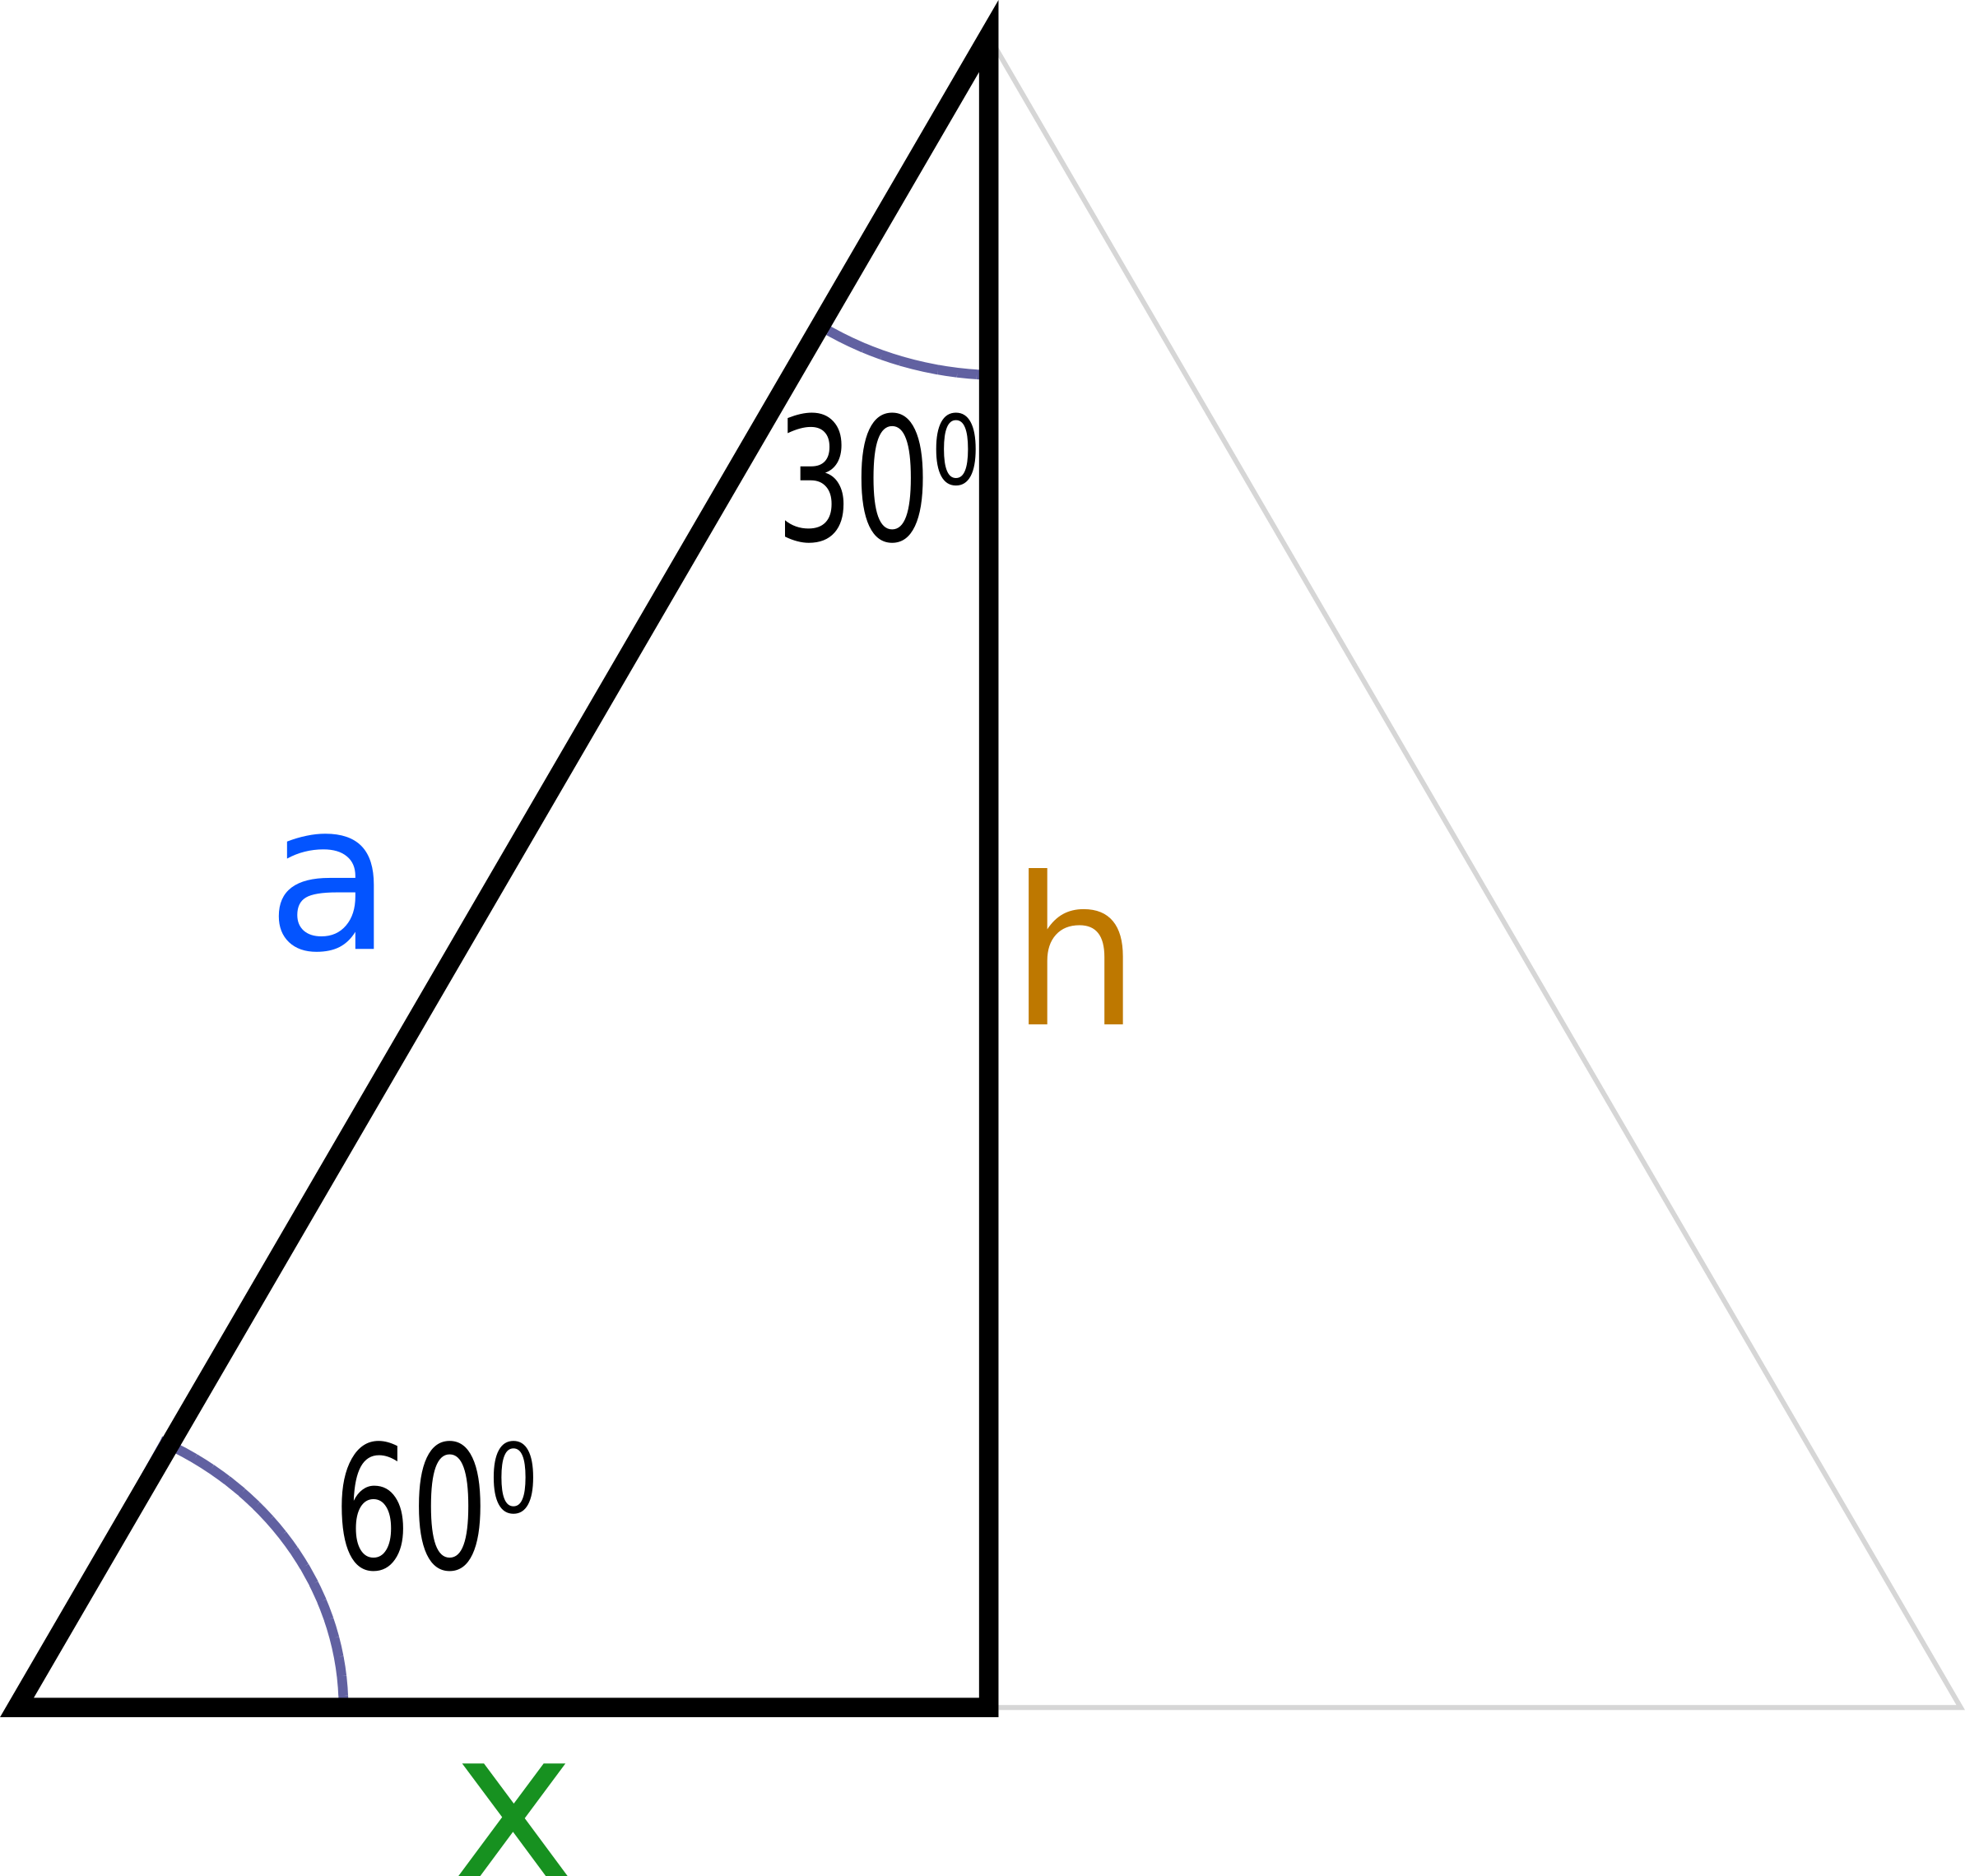
\includegraphics[width=4cm]{tals/plani/img/gleichseitigesDreieck.png}} &
  $\begin{array}{ll}
    x=& \frac{a}{2}                     \\
    h=& \sqrt{3}\cdot{}x                \\
    h=& \frac{\sqrt{3}}{2}\cdot{}a
  \end{array}$ \\

  \hline
  \raisebox{-24mm}{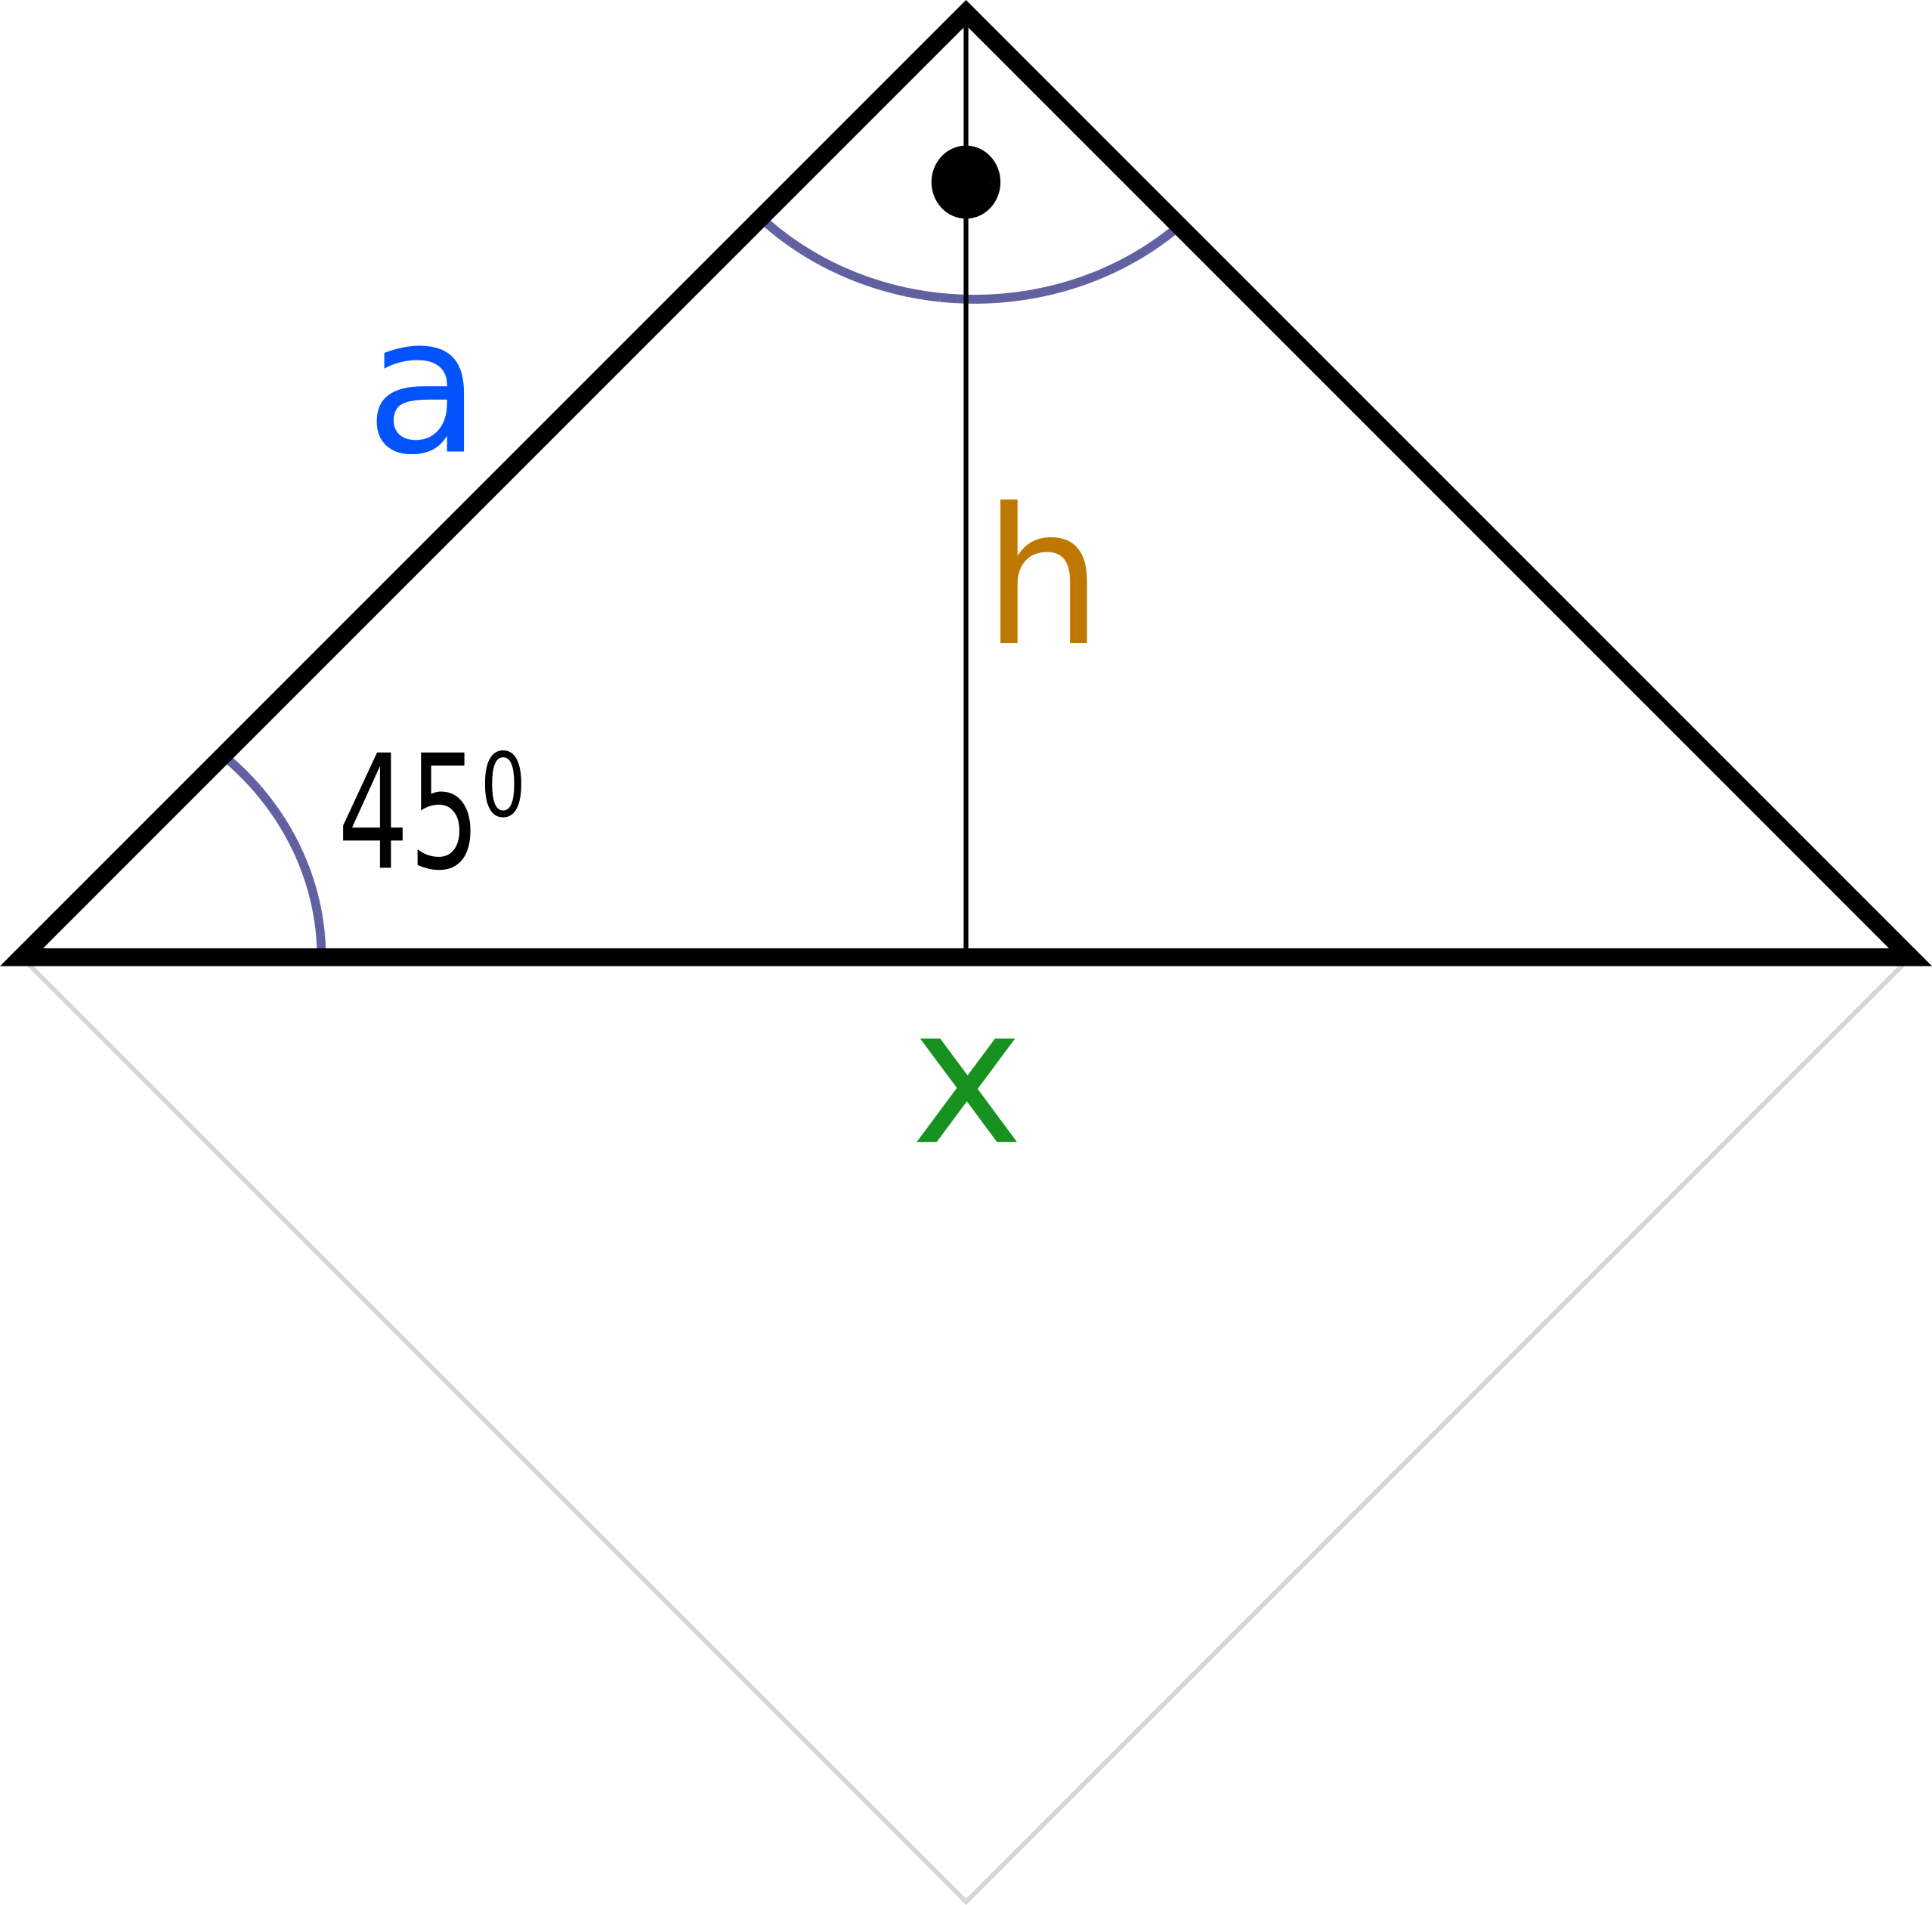
\includegraphics[width=5cm]{tals/plani/img/halbesQuadrat.png}} &
  $\begin{array}{ll}
    x=& \sqrt{2}\cdot{}a            \\
    h=& \frac{x}{2}                 \\
    h=& \frac{\sqrt{2}}{2} \cdot{} a\\
    a=& \sqrt{2}\cdot{}h
  \end{array}$ 
  \\
  
  \hline
\end{tabular} 
\renewcommand{\arraystretch}{1}

\TALS{Siehe auch \cite{frommenwiler18geom} S. 25 Kapitel 1.2.2}

\end{samepage}


\subsection*{Aufgaben}
\TALSGeomAadB{25}{68. 70. 72. 73.}

\GESOAadB{???}{???}
\newpage
